% Prof. Dr. Ausberto S. Castro Vera
% UENF - CCT - LCMAT - Curso de Ci\^{e}ncia da Computa\c{c}\~{a}o
% Campos, RJ,  2023 
% Disciplina: An\'{a}lise e Projeto de Sistemas
% Aluno: 

\chapterimage{analise.png} % Table of contents heading image
\chapter{Etapa de An\'{a}lise}


\section{Requisitos do Sistema}

\subsubsection{Requisito 1: Controle de Estoque}
\textbf{Definição:} O sistema deve permitir o controle de estoque de motos e peças de reposição, monitorando a quantidade atual disponível, entrada e saída de itens.
\\
\textbf{Especificação:}
\begin{itemize}
	\item 1.1. Manter um registro atualizado dos itens em estoque.
	\item 1.2. Registrar a entrada de novos itens no estoque.
	\item 1.3. Registrar a saída de itens do estoque, seja por vendas ou outras razões.
	\item 1.4. Alertar quando a quantidade de um item atingir um nível mínimo.
\end{itemize}

\subsubsection{Requisito 2: Impressão de Relatórios}
\textbf{Definição:} O sistema deve possibilitar a geração e impressão de relatórios, como relatórios de vendas, inventário de estoque e desempenho do sistema.
\\
\textbf{Especificação:}
\begin{itemize}
	\item 2.1. Oferecer opções para selecionar o tipo de relatório desejado.
	\item 2.2. Gerar o relatório com base nos dados armazenados no sistema.
	\item 2.3. Permitir visualizar o relatório antes da impressão.
	\item 2.4. Disponibilizar a opção de imprimir o relatório em uma impressora designada.
\end{itemize}

\subsubsection{Requisito 3: Gestão de Vendas}
\textbf{Definição:} O sistema deve permitir a realização de vendas de motos e peças de reposição, registrando informações do cliente, produtos vendidos e valores.
\\
\textbf{Especificação:}
\begin{itemize}
	\item 3.1. Registrar informações do cliente, como nome, contato e endereço.
	\item 3.2. Selecionar produtos a serem vendidos, incluindo motos e peças de reposição.
	\item 3.3. Calcular o valor total da venda com base nos produtos selecionados.
	\item 3.4. Emitir um recibo para o cliente após a conclusão da venda.
\end{itemize}

\subsubsection{Requisito 4: Cadastro de Clientes}
\textbf{Definição:} O sistema deve permitir o cadastro e gerenciamento de informações de clientes, incluindo nome, contato e histórico de compras.
\\
\textbf{Especificação:}
\begin{itemize}
	\item 4.1. Inserir e armazenar informações do cliente no banco de dados.
	\item 4.2. Atualizar dados de clientes existentes conforme necessário.
	\item 4.3. Exibir o histórico de compras de um cliente quando solicitado.
\end{itemize}

\subsubsection{Requisito 5: Cadastro de Motos}
\textbf{Definição:} O sistema deve permitir o cadastro de informações detalhadas sobre motos disponíveis para venda, incluindo modelo, marca, preço e especificações técnicas.
\\
\textbf{Especificação:}
\begin{itemize}
	\item 5.1. Registrar informações completas sobre cada modelo de moto disponível.
	\item 5.2. Associar preços correspondentes a cada moto.
	\item 5.3. Incluir especificações técnicas, como potência do motor e capacidade do tanque.
\end{itemize}

\subsubsection{Requisito 6: Acesso ao Sistema}
\textbf{Definição:} O sistema deve fornecer autenticação segura para garantir que apenas usuários autorizados possam acessá-lo.
\\
\textbf{Especificação:}
\begin{itemize}
	\item 6.1. Apresentar uma tela de login para entrada no sistema.
	\item 6.2. Solicitar nome de usuário e senha para autenticação.
	\item 6.3. Verificar as credenciais fornecidas em relação aos registros de usuários autorizados.
	\item 6.4. Conceder acesso ao sistema somente após a autenticação bem-sucedida.
\end{itemize}

\subsubsection{Requisito 7: Controle de Acesso}
\textbf{Definição:} O sistema deve permitir a definição de diferentes níveis de acesso para usuários, controlando quais recursos e funcionalidades eles podem utilizar.
\\
\textbf{Especificação:}
\begin{itemize}
	\item 7.1. Criar perfis de usuário com níveis de acesso específicos.
	\item 7.2. Associar cada usuário a um perfil de acesso.
	\item 7.3. Restringir o acesso a determinadas áreas do sistema com base no perfil do usuário.
\end{itemize}

\subsubsection{Requisito 8: Registro de Manutenção}
\textbf{Definição:} O sistema deve permitir o registro de manutenções realizadas em motos, incluindo detalhes sobre serviços, peças substituídas e custos.
\\
\textbf{Especificação:}
\begin{itemize}
	\item 8.1. Registrar detalhes da manutenção, como data, tipo de serviço e peças envolvidas.
	\item 8.2. Incluir o custo total da manutenção.
	\item 8.3. Associar a manutenção a uma moto específica para histórico de manutenção.
\end{itemize}

\subsubsection{Requisito 9: Reservas de Serviço}
\textbf{Definição:} O sistema deve permitir que os clientes façam reservas para serviços de manutenção e reparo em suas motos.
\\
\textbf{Especificação:}
\begin{itemize}
	\item 9.1. Aceitar solicitações de reserva de serviço dos clientes.
	\item 9.2. Agendar datas e horários para as reservas.
	\item 9.3. Notificar os clientes sobre datas e horários agendados.
	\item 9.4. Registrar detalhes sobre os serviços de manutenção solicitados.
\end{itemize}

\subsubsection{Requisito 10: Painel de Administração}
\textbf{Definição:} O sistema deve incluir um painel de administração que permita aos administradores gerenciar usuários, produtos, vendas e relatórios.
\\
\textbf{Especificação:}
\begin{itemize}
	\item 10.1. Fornecer acesso exclusivo a administradores autorizados.
	\item 10.2. Permitir adicionar, editar e excluir registros de usuários e produtos.
	\item 10.3. Facilitar a geração de relatórios sobre vendas e desempenho.
\end{itemize}

\subsubsection{Requisito 11: Notificações de Estoque}
\textbf{Definição:} O sistema deve ser capaz de enviar notificações aos administradores quando a quantidade de um item em estoque atingir um nível mínimo.
\\
\textbf{Especificação:}
\begin{itemize}
	\item 11.1. Monitorar continuamente a quantidade de itens em estoque.
	\item 11.2. Enviar notificações por email ou mensagem interna aos administradores quando necessário.
	\item 11.3. Incluir informações sobre o item e a quantidade atual no aviso.
\end{itemize}

\subsubsection{Requisito 12: Histórico de Vendas}
\textbf{Definição:} O sistema deve manter um registro histórico de todas as transações de vendas, permitindo consulta e análise.
\\
\textbf{Especificação:}
\begin{itemize}
	\item 12.1. Armazenar informações detalhadas sobre cada venda, incluindo data, produtos vendidos e valores.
	\item 12.2. Oferecer uma função de pesquisa para recuperar vendas específicas com base em critérios como data ou cliente.
\end{itemize}

\subsubsection{Requisito 13: Controle de Avarias}
\textbf{Definição:} O sistema deve permitir o registro de motos danificadas ou com defeito, incluindo detalhes sobre o problema e ações tomadas.
\\
\textbf{Especificação:}
\begin{itemize}
	\item 13.1. Registrar informações sobre a moto avariada, como modelo e número de série.
	\item 13.2. Descrever o problema ou defeito encontrado na moto.
	\item 13.3. Registrar ações de reparo ou manutenção realizadas na moto.
\end{itemize}

\subsubsection{Requisito 14: Promoções e Descontos}
\textbf{Definição:} O sistema deve permitir a criação e gerenciamento de promoções e descontos em produtos, a fim de atrair clientes.
\\
\textbf{Especificação:}
\begin{itemize}
	\item 14.1. Criar promoções com descontos específicos em motos ou peças de reposição.
	\item 14.2. Associar promoções a produtos específicos.
	\item 14.3. Exibir os preços promocionais nos produtos durante o período de promoção.
\end{itemize}

\subsubsection{Requisito 15: Integração de Pagamento Online}
\textbf{Definição:} O sistema deve oferecer a opção de pagamento online para os clientes que desejam comprar produtos pela internet.
\\
\textbf{Especificação:}
\begin{itemize}
	\item 15.1. Integrar um sistema de pagamento seguro, como cartões de crédito ou PayPal.
	\item 15.2. Permitir que os clientes escolham a opção de pagamento online durante o checkout.
	\item 15.3. Garantir que as transações online sejam seguras e protegidas contra fraudes.
\end{itemize}

\subsubsection{Requisito 16: Gestão de Fornecedores}
\textbf{Definição:} O sistema deve incluir um módulo de gestão de fornecedores para rastrear informações de fornecedores, pedidos e prazos de entrega.
\\
\textbf{Especificação:}
\begin{itemize}
	\item 16.1. Manter um registro de fornecedores, incluindo nome, contato e informações de pagamento.
	\item 16.2. Registrar pedidos de produtos a fornecedores.
	\item 16.3. Monitorar prazos de entrega e receber notificações sobre atrasos.
\end{itemize}

\subsubsection{Requisito 17: Suporte Multilíngue}
\textbf{Definição:} O sistema deve ser capaz de oferecer suporte a múltiplos idiomas, permitindo que os clientes escolham o idioma de sua preferência.
\\
\textbf{Especificação:}
\begin{itemize}
	\item 17.1. Disponibilizar uma lista de idiomas suportados para os clientes.
	\item 17.2. Permitir que os clientes selecionem seu idioma preferido no sistema.
	\item 17.3. Traduzir automaticamente o conteúdo do sistema para o idioma escolhido pelo cliente.
\end{itemize}

\subsubsection{Requisito 18: Relatórios de Desempenho}
\textbf{Definição:} O sistema deve gerar relatórios de desempenho que incluam métricas como vendas mensais, estoque atual e análises de tendências.
\\
\textbf{Especificação:}
\begin{itemize}
	\item 18.1. Criar relatórios automáticos que apresentem informações relevantes sobre o desempenho do negócio.
	\item 18.2. Incluir gráficos e gráficos para visualização de dados.
	\item 18.3. Permitir que os administradores personalizem os relatórios de acordo com suas necessidades.
\end{itemize}

\subsubsection{Requisito 19: Backup e Recuperação de Dados}
\textbf{Definição:} O sistema deve implementar rotinas de backup regulares para proteger os dados do sistema contra perdas ou danos.
\\
\textbf{Especificação:}
\begin{itemize}
	\item 19.1. Realizar backups automáticos diários de todos os dados do sistema.
	\item 19.2. Armazenar cópias de backup em locais seguros e fora das instalações.
	\item 19.3. Estabelecer procedimentos de recuperação de dados para restaurar informações em caso de falha.
\end{itemize}

\subsubsection{Requisito 20: Atualizações de Software}
\textbf{Definição:} O sistema deve permitir atualizações de software para adicionar novos recursos, corrigir bugs e melhorar a segurança.
\\
\textbf{Especificação:}
\begin{itemize}
	\item 20.1. Notificar os administradores sobre novas atualizações disponíveis.
	\item 20.2. Facilitar o processo de atualização, permitindo que os administradores apliquem atualizações com facilidade.
	\item 20.3. Realizar testes rigorosos em atualizações antes de implantá-las no ambiente de produção.
\end{itemize}

\subsubsection{Requisito 21: Autenticação de Dois Fatores}
\textbf{Definição:} O sistema deve oferecer autenticação de dois fatores (2FA) como uma opção de segurança adicional para os usuários.
\\
\textbf{Especificação:}
\begin{itemize}
	\item 21.1. Permitir que os usuários habilitem a autenticação de dois fatores em suas contas.
	\item 21.2. Utilizar métodos de autenticação, como códigos de verificação ou notificações por aplicativo móvel.
	\item 21.3. Exigir a autenticação de dois fatores sempre que os usuários fizerem login em dispositivos não reconhecidos.
\end{itemize}

\subsubsection{Requisito 22: Gestão de Devoluções}
\textbf{Definição:} O sistema deve permitir que os clientes solicitem devoluções de produtos e rastreiem o status dessas devoluções.
\\
\textbf{Especificação:}
\begin{itemize}
	\item 22.1. Oferecer aos clientes a opção de iniciar solicitações de devolução através do sistema.
	\item 22.2. Registrar detalhes sobre o motivo da devolução e os produtos envolvidos.
	\item 22.3. Manter um histórico das solicitações de devolução e seu status (pendente, aprovado, concluído, etc.).
\end{itemize}

\subsubsection{Requisito 23: Gestão de Créditos e Reembolsos}
\textbf{Definição:} O sistema deve suportar a emissão de créditos e reembolsos aos clientes quando necessário.
\\
\textbf{Especificação:}
\begin{itemize}
	\item 23.1. Permitir que os administradores emitam créditos ou processem reembolsos para clientes de acordo com a política da empresa.
	\item 23.2. Manter um registro detalhado de todas as transações de créditos e reembolsos.
	\item 23.3. Notificar automaticamente os clientes sobre a emissão de créditos ou reembolsos.
\end{itemize}

\subsubsection{Requisito 24: Integração com Plataformas de Mídia Social}
\textbf{Definição:} O sistema deve permitir a integração com plataformas de mídia social para compartilhamento de produtos e promoções.
\\
\textbf{Especificação:}
\begin{itemize}
	\item 24.1. Incluir botões de compartilhamento para redes sociais em páginas de produtos.
	\item 24.2. Permitir que os clientes compartilhem produtos e promoções em suas contas de mídia social.
	\item 24.3. Rastrear métricas de compartilhamento e engajamento social.
\end{itemize}

\subsubsection{Requisito 25: Personalização de Produtos}
\textbf{Definição:} O sistema deve permitir que os clientes personalizem produtos, como motos, escolhendo cores, acessórios, etc.
\\
\textbf{Especificação:}
\begin{itemize}
	\item 25.1. Oferecer uma interface de personalização intuitiva para os clientes escolherem opções de personalização.
	\item 25.2. Atualizar o preço automaticamente com base nas opções de personalização escolhidas.
	\item 25.3. Transmitir as opções de personalização aos departamentos de produção e estoque para atender às solicitações dos clientes.
\end{itemize}

\subsubsection{Requisito 26: Comparação de Produtos}
\textbf{Definição:} O sistema deve permitir que os clientes comparem especificações e preços de diferentes motos ou produtos.
\\
\textbf{Especificação:}
\begin{itemize}
	\item 26.1. Exibir uma tabela de comparação que permite aos clientes selecionar várias motos ou produtos para comparação.
	\item 26.2. Mostrar informações detalhadas, como especificações técnicas, preço e disponibilidade, lado a lado para facilitar a comparação.
\end{itemize}

\subsubsection{Requisito 27: Suporte a Programas de Fidelidade}
\textbf{Definição:} O sistema deve oferecer suporte a programas de fidelidade, permitindo que os clientes acumulem pontos e recebam recompensas.
\\
\textbf{Especificação:}
\begin{itemize}
	\item 27.1. Permitir que os clientes se inscrevam em programas de fidelidade.
	\item 27.2. Atribuir pontos aos clientes com base em suas compras e interações.
	\item 27.3. Oferecer recompensas, descontos ou produtos gratuitos em troca de pontos acumulados.
\end{itemize}

\subsubsection{Requisito 28: Acesso a Relatórios Financeiros}
\textbf{Definição:} O sistema deve fornecer acesso a relatórios financeiros detalhados para análise e tomada de decisões.
\\
\textbf{Especificação:}
\begin{itemize}
	\item 28.1. Gerar relatórios financeiros, incluindo balanços, demonstrações de resultados e análises de fluxo de caixa.
	\item 28.2. Disponibilizar relatórios atualizados em tempo real.
	\item 28.3. Restringir o acesso a relatórios financeiros a usuários autorizados, como contadores e gerentes financeiros.
\end{itemize}

\subsubsection{Requisito 29: Configuração de Impostos e Taxas}
\textbf{Definição:} O sistema deve permitir que os administradores configurem impostos e taxas aplicáveis a vendas e transações.
\\
\textbf{Especificação:}
\begin{itemize}
	\item 29.1. Oferecer uma interface de configuração para definir taxas de imposto por região ou país.
	\item 29.2. Aplicar automaticamente impostos e taxas aos produtos com base nas configurações definidas.
	\item 29.3. Incluir a taxa de imposto no processo de checkout para transparência para os clientes.
\end{itemize}

\subsubsection{Requisito 30: Suporte a Chat Online}
\textbf{Definição:} O sistema deve oferecer suporte a um sistema de chat online para que os clientes possam obter assistência em tempo real.
\\
\textbf{Especificação:}
\begin{itemize}
	\item 30.1. Integrar um sistema de chat online que permita aos clientes iniciar conversas com agentes de suporte.
	\item 30.2. Rastrear o histórico de conversas para referência futura.
	\item 30.3. Notificar os agentes de suporte quando os clientes necessitarem de assistência.
\end{itemize}

\subsubsection{Requisito 31: Gestão de Motos Usadas}
\textbf{Definição:} O sistema deve permitir o cadastramento, venda e gerenciamento de motos usadas.
\\
\textbf{Especificação:}
\begin{itemize}
	\item 31.1. Oferecer a opção de cadastrar motos usadas no sistema, incluindo informações como modelo, ano, quilometragem, etc.
	\item 31.2. Permitir que os clientes visualizem e comprem motos usadas através da plataforma.
	\item 31.3. Manter um registro detalhado de todas as motos usadas, incluindo histórico de manutenção e preço.
\end{itemize}

\subsubsection{Requisito 32: Integração com Sistemas de Pagamento}
\textbf{Definição:} O sistema deve integrar-se a sistemas de pagamento online para facilitar transações financeiras.
\\
\textbf{Especificação:}
\begin{itemize}
	\item 32.1. Oferecer opções de pagamento online, como cartões de crédito, PayPal, etc.
	\item 32.2. Garantir que todas as transações financeiras sejam seguras e protegidas.
	\item 32.3. Registrar detalhes de transações financeiras para fins de contabilidade.
\end{itemize}

\subsubsection{Requisito 33: Gerenciamento de Ofertas e Promoções}
\textbf{Definição:} O sistema deve permitir a criação e gerenciamento de ofertas, descontos e promoções especiais.
\\
\textbf{Especificação:}
\begin{itemize}
	\item 33.1. Permitir que os administradores criem ofertas especiais, como descontos em produtos ou pacotes promocionais.
	\item 33.2. Definir regras de validade para as ofertas, incluindo datas de início e término.
	\item 33.3. Exibir ofertas especiais para os clientes de forma proeminente no site.
\end{itemize}

\subsubsection{Requisito 34: Rastreamento de Entrega de Pedidos}
\textbf{Definição:} O sistema deve permitir que os clientes rastreiem o status e a entrega de seus pedidos.
\\
\textbf{Especificação:}
\begin{itemize}
	\item 34.1. Fornecer informações de rastreamento para cada pedido, incluindo data de envio, transportadora e previsão de entrega.
	\item 34.2. Enviar notificações por e-mail ou SMS aos clientes com atualizações sobre o status da entrega.
	\item 34.3. Permitir que os clientes entrem em contato com a transportadora em caso de problemas na entrega.
\end{itemize}

\subsubsection{Requisito 35: Suporte a Múltiplos Idiomas}
\textbf{Definição:} O sistema deve oferecer suporte a múltiplos idiomas para atender a uma base de clientes global.
\\
\textbf{Especificação:}
\begin{itemize}
	\item 35.1. Permitir que os clientes escolham seu idioma preferido ao acessar o site.
	\item 35.2. Traduzir automaticamente o conteúdo do site com base na seleção do idioma do cliente.
	\item 35.3. Fornecer uma interface de administração para adicionar novos idiomas e gerenciar traduções.
\end{itemize}

\subsubsection{Requisito 36: Gerenciamento de Avaliações e Comentários}
\textbf{Definição:} O sistema deve permitir que os clientes avaliem produtos e deixem comentários.
\\
\textbf{Especificação:}
\begin{itemize}
	\item 36.1. Permitir que os clientes avaliem produtos em uma escala de classificação.
	\item 36.2. Permitir que os clientes escrevam comentários detalhados sobre produtos.
	\item 36.3. Moderar e aprovar comentários antes que eles sejam exibidos publicamente.
\end{itemize}

\subsubsection{Requisito 37: Histórico de Compras}
\textbf{Definição:} O sistema deve manter um histórico completo de todas as compras dos clientes.
\\
\textbf{Especificação:}
\begin{itemize}
	\item 37.1. Armazenar registros de todas as compras, incluindo produtos adquiridos, data e valor.
	\item 37.2. Permitir que os clientes acessem seu histórico de compras a qualquer momento.
	\item 37.3. Usar o histórico de compras para oferecer recomendações personalizadas de produtos.
\end{itemize}

\subsubsection{Requisito 38: Backup e Recuperação de Dados}
\textbf{Definição:} O sistema deve implementar um sistema de backup regular e recuperação de dados em caso de falhas.
\\
\textbf{Especificação:}
\begin{itemize}
	\item 38.1. Realizar backups diários de todos os dados do sistema.
	\item 38.2. Armazenar backups em locais seguros e fora das instalações.
	\item 38.3. Ter procedimentos de recuperação de dados eficazes em caso de perda de dados.
\end{itemize}

\subsubsection{Requisito 39: Acessibilidade}
\textbf{Definição:} O sistema deve ser acessível a todos os usuários, incluindo aqueles com deficiências visuais ou motoras.
\\
\textbf{Especificação:}
\begin{itemize}
	\item 39.1. Seguir diretrizes de acessibilidade da web, como WCAG, para garantir que o sistema seja navegável por leitores de tela.
	\item 39.2. Fornecer opções de aumento de tamanho de fonte e contraste para usuários com deficiências visuais.
	\item 39.3. Garantir que todas as funcionalidades possam ser operadas com o uso de teclado para usuários com mobilidade reduzida.
\end{itemize}

\subsubsection{Requisito 40: Análise de Dados do Cliente}
\textbf{Definição:} O sistema deve coletar dados do cliente para análise e personalização de experiência.
\\
\textbf{Especificação:}
\begin{itemize}
	\item 40.1. Coletar dados de navegação, como páginas visitadas e produtos visualizados.
	\item 40.2. Analisar os dados do cliente para oferecer recomendações personalizadas de produtos.
	\item 40.3. Garantir a privacidade e segurança dos dados do cliente de acordo com as regulamentações de proteção de dados.
\end{itemize}

\subsubsection{Requisito 41: Suporte a Chat Online}
\textbf{Definição:} O sistema deve oferecer suporte a um serviço de chat online para atendimento ao cliente em tempo real.
\\
\textbf{Especificação:}
\begin{itemize}
	\item 41.1. Integrar um sistema de chat em tempo real para que os clientes possam entrar em contato com a equipe de suporte.
	\item 41.2. Permitir que os clientes vejam a disponibilidade dos agentes de suporte.
	\item 41.3. Registrar o histórico das conversas de chat para referência futura.
\end{itemize}

\subsubsection{Requisito 42: Relatórios de Vendas}
\textbf{Definição:} O sistema deve gerar relatórios detalhados sobre as vendas e o desempenho do negócio.
\\
\textbf{Especificação:}
\begin{itemize}
	\item 42.1. Gerar relatórios diários, semanais e mensais de vendas, incluindo dados como total de vendas, produtos mais vendidos e receita.
	\item 42.2. Permitir que os administradores personalizem os relatórios de acordo com suas necessidades.
	\item 42.3. Exportar relatórios em formatos como PDF e CSV.
\end{itemize}

\subsubsection{Requisito 43: Notificações por E-mail}
\textbf{Definição:} O sistema deve enviar notificações por e-mail para informar os clientes sobre promoções, atualizações e transações.
\\
\textbf{Especificação:}
\begin{itemize}
	\item 43.1. Coletar informações de contato dos clientes para fins de comunicação por e-mail.
	\item 43.2. Enviar notificações sobre ofertas especiais, confirmações de pedidos e atualizações de produtos.
	\item 43.3. Permitir que os clientes escolham suas preferências de recebimento de e-mails.
\end{itemize}

\subsubsection{Requisito 44: Fórum da Comunidade}
\textbf{Definição:} O sistema deve oferecer um fórum de comunidade para que os clientes possam discutir produtos e compartilhar experiências.
\\
\textbf{Especificação:}
\begin{itemize}
	\item 44.1. Implementar um fórum de discussão onde os clientes possam criar tópicos e responder a posts.
	\item 44.2. Moderar o fórum para garantir que as discussões sejam respeitosas e construtivas.
	\item 44.3. Fornecer um sistema de reputação para reconhecer membros ativos da comunidade.
\end{itemize}

\subsubsection{Requisito 45: Personalização de Produtos}
\textbf{Definição:} O sistema deve permitir que os clientes personalizem produtos antes de fazer uma compra.
\\
\textbf{Especificação:}
\begin{itemize}
	\item 45.1. Oferecer ferramentas de personalização, como escolha de cores, adição de monogramas, etc.
	\item 45.2. Atualizar o preço automaticamente com base nas opções de personalização escolhidas.
	\item 45.3. Garantir que as opções de personalização sejam claras e intuitivas para os clientes.
\end{itemize}

\subsubsection{Requisito 46: Integração de Redes Sociais}
\textbf{Definição:} O sistema deve integrar-se a redes sociais para permitir que os clientes compartilhem produtos e conteúdo.
\\
\textbf{Especificação:}
\begin{itemize}
	\item 46.1. Incluir botões de compartilhamento para redes sociais em páginas de produtos e conteúdo.
	\item 46.2. Permitir que os clientes compartilhem suas compras e avaliações em suas próprias redes sociais.
	\item 46.3. Acompanhar métricas de compartilhamento social para avaliar o impacto nas vendas.
\end{itemize}

\subsubsection{Requisito 47: Reserva de Produtos}
\textbf{Definição:} O sistema deve permitir que os clientes reservem produtos por um período limitado antes de fazer a compra.
\\
\textbf{Especificação:}
\begin{itemize}
	\item 47.1. Oferecer a opção de reserva para produtos com estoque limitado.
	\item 47.2. Definir um período de reserva, após o qual o produto será liberado para outros clientes.
	\item 47.3. Notificar os clientes sobre o status de suas reservas e fornecer instruções para conclusão da compra.
\end{itemize}

\subsubsection{Requisito 48: Controle de Acesso Hierárquico}
\textbf{Definição:} O sistema deve suportar uma estrutura de controle de acesso com níveis hierárquicos para administradores e funcionários.
\\
\textbf{Especificação:}
\begin{itemize}
	\item 48.1. Definir diferentes níveis de acesso, como administrador, gerente e funcionário.
	\item 48.2. Garantir que os administradores tenham acesso total a todas as funcionalidades do sistema.
	\item 48.3. Restringir o acesso de funcionários a funcionalidades específicas de acordo com suas atribuições.
\end{itemize}

\subsubsection{Requisito 49: Suporte a Dispositivos Móveis}
\textbf{Definição:} O sistema deve ser responsivo e suportar dispositivos móveis, como smartphones e tablets.
\\
\textbf{Especificação:}
\begin{itemize}
	\item 49.1. Garantir que o site seja totalmente funcional e de fácil utilização em dispositivos móveis.
	\item 49.2. Adaptar automaticamente a interface do usuário de acordo com o tamanho da tela.
	\item 49.3. Testar regularmente a compatibilidade com os principais navegadores móveis.
\end{itemize}

\subsubsection{Requisito 50: Integração com Sistema de CRM}
\textbf{Definição:} O sistema deve integrar-se a um sistema de gerenciamento de relacionamento com o cliente (CRM) para melhorar o atendimento ao cliente.
\\
\textbf{Especificação:}
\begin{itemize}
	\item 50.1. Sincronizar dados de clientes e histórico de interações com o sistema CRM.
	\item 50.2. Permitir que a equipe de atendimento ao cliente acesse informações do CRM durante interações com os clientes.
	\item 50.3. Automatizar o registro de novos clientes no sistema CRM.
\end{itemize}

\subsubsection{Requisito 51: Proteção contra Vírus e Malware}
\textbf{Definição:} O sistema deve implementar medidas de segurança para proteger contra vírus e malware.
\\
\textbf{Especificação:}
\begin{itemize}
	\item 51.1. Utilizar software antivírus atualizado para escanear arquivos e sistemas regularmente.
	\item 51.2. Implementar filtros de e-mail para evitar a propagação de arquivos maliciosos.
	\item 51.3. Manter sistemas operacionais e software de servidor atualizados com patches de segurança.
\end{itemize}

\subsubsection{Requisito 52: Criptografia de Dados Sensíveis}
\textbf{Definição:} O sistema deve criptografar dados sensíveis armazenados e transmitidos para garantir sua confidencialidade.
\\
\textbf{Especificação:}
\begin{itemize}
	\item 52.1. Utilizar protocolos de criptografia (por exemplo, SSL/TLS) para proteger a transmissão de dados pela rede.
	\item 52.2. Armazenar senhas e informações de pagamento dos clientes em formato criptografado.
	\item 52.3. Implementar criptografia de dados em repouso nos bancos de dados para proteger informações sensíveis.
\end{itemize}

\subsubsection{Requisito 53: Backup Regular de Bancos de Dados}
\textbf{Definição:} O sistema deve realizar backups regulares dos bancos de dados para garantir a recuperação de dados em caso de falhas.
\\
\textbf{Especificação:}
\begin{itemize}
	\item 53.1. Agendar backups automáticos diários dos bancos de dados.
	\item 53.2. Armazenar cópias de backup em local seguro e fora das instalações físicas.
	\item 53.3. Testar periodicamente a restauração de dados a partir dos backups para garantir a eficácia do processo.
\end{itemize}

\subsubsection{Requisito 54: Monitoramento de Segurança de Servidores}
\textbf{Definição:} O sistema deve implementar um sistema de monitoramento contínuo para identificar e responder a possíveis ameaças de segurança nos servidores.
\\
\textbf{Especificação:}
\begin{itemize}
	\item 54.1. Utilizar ferramentas de monitoramento de segurança para rastrear atividades suspeitas nos servidores.
	\item 54.2. Configurar alertas para notificar a equipe de segurança sobre atividades anômalas.
	\item 54.3. Manter registros de auditoria detalhados para fins de investigação de segurança.
\end{itemize}

\subsubsection{Requisito 55: Tolerância a Falhas em Servidores}
\textbf{Definição:} O sistema deve ser projetado com tolerância a falhas para garantir a disponibilidade contínua, mesmo em caso de falhas de hardware ou software.
\\
\textbf{Especificação:}
\begin{itemize}
	\item 55.1. Configurar servidores em clusters para permitir a transferência automática de carga em caso de falhas.
	\item 55.2. Implementar balanceamento de carga para distribuir o tráfego de forma equitativa entre os servidores.
	\item 55.3. Manter sistemas redundantes para componentes críticos, como fontes de alimentação e discos rígidos.
\end{itemize}

\subsubsection{Requisito 56: Gerenciamento de Patches de Segurança}
\textbf{Definição:} O sistema deve estabelecer um processo formal para gerenciamento de patches de segurança.
\\
\textbf{Especificação:}
\begin{itemize}
	\item 56.1. Avaliar regularmente os patches de segurança disponíveis para sistemas operacionais e software de servidor.
	\item 56.2. Estabelecer um cronograma para aplicação de patches de segurança, minimizando o tempo de inatividade.
	\item 56.3. Testar patches em ambiente de desenvolvimento antes de aplicá-los em produção.
\end{itemize}

\subsubsection{Requisito 57: Autenticação de Dois Fatores (2FA)}
\textbf{Definição:} O sistema deve oferecer a opção de autenticação de dois fatores para aumentar a segurança das contas de usuário.
\\
\textbf{Especificação:}
\begin{itemize}
	\item 57.1. Permitir que os usuários ativem a autenticação de dois fatores em suas contas.
	\item 57.2. Implementar métodos de autenticação secundária, como códigos de verificação ou autenticação por aplicativo.
	\item 57.3. Exigir a autenticação de dois fatores para ações sensíveis, como alterações de senha ou informações de pagamento.
\end{itemize}

\subsubsection{Requisito 58: Auditoria de Acesso ao Sistema}
\textbf{Definição:} O sistema deve registrar e monitorar todas as atividades de acesso ao sistema para fins de auditoria.
\\
\textbf{Especificação:}
\begin{itemize}
	\item 58.1. Registrar detalhes de cada acesso ao sistema, incluindo data, hora, endereço IP e usuário.
	\item 58.2. Manter logs de auditoria por um período especificado de acordo com as regulamentações aplicáveis.
	\item 58.3. Implementar políticas de retenção de logs para otimizar o uso de armazenamento.
\end{itemize}

\subsubsection{Requisito 59: Restrição de Acesso a Dados Sensíveis}
\textbf{Definição:} O sistema deve restringir o acesso a dados sensíveis, permitindo que apenas usuários autorizados visualizem e modifiquem essas informações.
\\
\textbf{Especificação:}
\begin{itemize}
	\item 59.1. Definir permissões de acesso com base nas funções e responsabilidades dos usuários.
	\item 59.2. Criar políticas de acesso que determinem quem pode visualizar, editar e excluir dados sensíveis.
	\item 59.3. Implementar mecanismos de controle de acesso, como autenticação e autorização, para garantir o cumprimento das políticas.
\end{itemize}

\subsubsection{Requisito 60: Testes de Penetração Regulares}
\textbf{Definição:} O sistema deve passar por testes de penetração regulares para identificar vulnerabilidades e avaliar a eficácia das medidas de segurança.
\\
\textbf{Especificação:}
\begin{itemize}
	\item 60.1. Contratar profissionais de segurança ou empresas especializadas para realizar testes de penetração.
	\item 60.2. Agendar testes de penetração em intervalos regulares, especialmente após alterações significativas no sistema.
	\item 60.3. Documentar e abordar todas as vulnerabilidades identificadas durante os testes.
\end{itemize}


\section{Stakeholders e Pontos de Vista}

Neste capítulo, exploraremos os principais stakeholders envolvidos no projeto do Sistema de Gerenciamento de Concessionárias de Motos e examinaremos suas perspectivas e necessidades em relação ao sistema. Identificar e compreender os stakeholders é fundamental para o sucesso do projeto, pois suas expectativas orientarão o desenvolvimento e a implementação do sistema.

\subsection{Principais Stakeholders}

Neste capítulo, exploraremos os principais stakeholders envolvidos no projeto do Sistema de Gerenciamento de Concessionárias de Motos e examinaremos em profundidade suas perspectivas, expectativas e necessidades em relação ao sistema. Identificar e compreender os stakeholders é de importância crítica para o sucesso do projeto, pois suas visões e demandas orientarão o desenvolvimento, implementação e melhoria contínua do sistema.

\subsubsection{1. Concessionárias de Motos}

\textbf{Pontos de Vista:} As concessionárias de motos representam os principais usuários do sistema. Eles estão profundamente interessados em um sistema que simplifique e aprimore o gerenciamento de inventário. Para eles, é crucial que o sistema permita um acompanhamento preciso das vendas, gestão de clientes, rastreamento de estoque e comunicação eficaz com seus clientes.

\subsubsection{2. Clientes}

\textbf{Pontos de Vista:} Os clientes, sendo a parte que interage diretamente com o sistema por meio das concessionárias, valorizam uma experiência de compra simplificada e eficiente. Eles esperam que o sistema forneça informações detalhadas e atualizadas sobre produtos, preços e disponibilidade. A facilidade de uso e a segurança durante o processo de compra são fatores críticos para sua satisfação.

\subsubsection{3. Equipe de Vendas}

\textbf{Pontos de Vista:} A equipe de vendas depende fortemente do sistema para melhorar seu desempenho. Eles necessitam de acesso instantâneo a informações de inventário, preços e histórico de compras dos clientes. O sistema deve auxiliá-los na criação de orçamentos, registro de vendas e fornecimento de dados que os capacitam a oferecer recomendações personalizadas e serviços de alta qualidade aos clientes.

\subsubsection{4. Gerentes de Concessionárias}

\textbf{Pontos de Vista:} Os gerentes de concessionárias buscam uma visão abrangente das operações do negócio. Eles dependem do sistema para gerar relatórios gerenciais detalhados que fornecem insights críticos sobre o desempenho financeiro, análises de vendas e tendências do mercado. Esses relatórios orientam suas decisões estratégicas e operacionais.

\subsubsection{5. Desenvolvedores e Equipe de TI}

\textbf{Pontos de Vista:} A equipe de desenvolvimento e TI é responsável pela implementação, manutenção e segurança contínua do sistema. Eles estão focados em garantir que a infraestrutura tecnológica seja robusta e escalável. Além disso, eles trabalham incansavelmente para implementar medidas de segurança eficazes, protegendo os dados sensíveis da concessionária e dos clientes. A estabilidade e a disponibilidade do sistema também estão no centro de suas preocupações.

\subsection{Pontos de Vista e Necessidades}

Aqui estão algumas das principais necessidades e expectativas dos stakeholders em relação ao sistema:

\subsubsection{Clientes:}

\begin{itemize}
	\item Acesso fácil a informações detalhadas sobre produtos e serviços.
	\item Processo de compra intuitivo, eficiente e seguro.
	\item Comunicação eficaz com a concessionária para consultas e suporte pós-venda.
\end{itemize}

\subsubsection{Equipe de Vendas:}

\begin{itemize}
	\item Acesso rápido e fácil a informações de inventário atualizadas.
	\item Capacidade de criar orçamentos, registrar vendas e gerenciar o relacionamento com os clientes.
	\item Histórico de compras dos clientes disponível para oferecer recomendações personalizadas.
\end{itemize}

\subsubsection{Gerentes de Concessionárias:}

\begin{itemize}
	\item Relatórios gerenciais detalhados para avaliação de desempenho e tomada de decisões informadas.
	\item Monitoramento constante das operações da concessionária, incluindo vendas, estoque e desempenho financeiro.
\end{itemize}

\subsubsection{Desenvolvedores e Equipe de TI:}

\begin{itemize}
	\item Infraestrutura tecnológica escalável, robusta e de alto desempenho.
	\item Implementação de medidas de segurança rigorosas para proteger os dados confidenciais.
	\item Manutenção proativa e suporte técnico contínuo para garantir a operação eficiente do sistema.
\end{itemize}

\subsection{Conclusão}

Compreender a fundo os stakeholders e suas perspectivas é de importância crítica para o sucesso do projeto do Sistema de Gerenciamento de Concessionárias de Motos. Ao considerar cuidadosamente as necessidades e expectativas de todas as partes envolvidas, podemos desenvolver um sistema que não apenas atenda às suas expectativas, mas também promova eficiência, segurança e satisfação para todos os usuários.


\section{Entrevista}

A realização de entrevistas é uma parte fundamental do processo de coleta de informações e requisitos para o sistema de gerenciamento de concessionárias de motos. As entrevistas permitem que a equipe de desenvolvimento obtenha uma compreensão mais profunda das necessidades e expectativas dos principais stakeholders envolvidos no projeto. Além disso, as entrevistas proporcionam a oportunidade de esclarecer dúvidas, identificar desafios potenciais e reunir insights valiosos.

\subsection{Seleção de Stakeholders}

Antes de conduzir as entrevistas, é essencial identificar e selecionar os stakeholders-chave que serão entrevistados. Os stakeholders são indivíduos ou grupos que têm um interesse direto ou indireto no sistema. Para este projeto, os seguintes grupos de stakeholders foram identificados como sendo de alta relevância:

\begin{itemize}
	\item \textbf{Concessionárias de Motos}: Os proprietários e funcionários das concessionárias desempenham um papel central, pois serão os principais usuários do sistema. Eles podem fornecer informações sobre processos de negócios existentes, necessidades específicas e expectativas em relação ao sistema.
	
	\item \textbf{Clientes}: Os clientes das concessionárias são uma parte fundamental do ecossistema. Suas opiniões e experiências podem influenciar diretamente o design do sistema, especialmente no que diz respeito à interface do usuário e à experiência do cliente.
	
	\item \textbf{Equipe de TI}: A equipe de tecnologia da informação das concessionárias desempenha um papel crucial na implementação e manutenção do sistema. Entender suas necessidades e requisitos técnicos é vital para o sucesso do projeto.
	
	\item \textbf{Gerentes de Concessionárias}: Os gerentes de concessionárias têm uma visão abrangente das operações e dos objetivos de negócios. Suas perspectivas estratégicas podem ajudar a moldar o escopo e os objetivos do sistema.
	
	\item \textbf{Fornecedores de Motos}: Para garantir uma integração eficaz com os fornecedores, é importante entrevistar representantes dessas empresas. Isso pode incluir discussões sobre sistemas de gerenciamento de cadeia de suprimentos.
\end{itemize}

\subsection{Planejamento das Entrevistas}

A fase de planejamento das entrevistas desempenha um papel fundamental no processo de análise e design do sistema de gerenciamento de concessionárias de motos. Um planejamento cuidadoso é essencial para garantir que o tempo e os recursos sejam utilizados de maneira eficaz e que as entrevistas atinjam seus objetivos.

\subsubsection{Definição de Objetivos Claros}

Antes de conduzir cada entrevista, estabelecemos objetivos claros e específicos. Isso envolve a definição de metas específicas para cada sessão de entrevista, garantindo que as perguntas sejam direcionadas para obter informações relevantes. Esses objetivos ajudam a manter o foco e a relevância das entrevistas, garantindo que as informações coletadas sejam úteis para o projeto.

\subsubsection{Agendamento Estratégico}

O agendamento das entrevistas é uma parte fundamental do planejamento. As entrevistas são marcadas de acordo com a disponibilidade dos stakeholders, considerando as agendas de funcionários da concessionária, gerentes e outros envolvidos no processo de vendas de motos. Um calendário é estabelecido para garantir que todas as partes interessadas tenham a oportunidade de serem ouvidas. Isso ajuda a otimizar a coleta de informações e a garantir a participação de todos os envolvidos.

\subsubsection{Roteiro de Entrevista Flexível}

Cada entrevista é conduzida com base em um roteiro de entrevista predefinido. Este roteiro inclui uma lista de perguntas e tópicos a serem abordados, mas também permite flexibilidade para explorar áreas emergentes durante a conversa. Isso significa que as entrevistas não são estritamente guiadas por um script, mas sim direcionadas para permitir que os stakeholders compartilhem suas visões e insights.

\subsubsection{Documentação Abrangente}

Durante as entrevistas, são utilizados métodos de documentação para garantir que nenhum detalhe seja perdido. Isso inclui gravações de áudio, notas escritas ou ambos, dependendo das preferências dos entrevistados. Essa abordagem de documentação minuciosa permite uma análise posterior aprofundada e garante que todas as informações coletadas sejam devidamente registradas.

O planejamento cuidadoso das entrevistas é uma etapa essencial para coletar informações valiosas dos stakeholders, que servirão como base para o projeto do sistema. Essa abordagem garante que as entrevistas sejam produtivas, eficientes e contribuam para o sucesso do sistema de gerenciamento de concessionárias de motos.

\subsection{Condução das Entrevistas}

Durante a fase de análise do sistema de gerenciamento de concessionárias de motos, foram realizadas entrevistas com os principais stakeholders envolvidos no projeto. Essas entrevistas tinham como objetivo coletar informações essenciais para entender as necessidades e expectativas dos usuários e partes interessadas.

Durante a condução das entrevistas, adotamos uma abordagem aberta e receptiva, garantindo que todos os participantes se sentissem à vontade para compartilhar suas opiniões e preocupações. Foram realizadas sessões com funcionários da concessionária, gerentes e outros envolvidos no processo de vendas de motos.

As perguntas abordaram uma variedade de tópicos, incluindo os desafios enfrentados no processo de venda, as preferências dos clientes, os procedimentos atuais e as expectativas em relação ao novo sistema. Além disso, foram feitas perguntas de acompanhamento para obter esclarecimentos e detalhes adicionais.

\subsection{Análise dos Resultados}

Após a conclusão das entrevistas, os dados coletados passaram por um processo de análise detalhada. O objetivo era identificar padrões, tendências e requisitos comuns a partir das informações fornecidas pelos stakeholders.

Foi evidente que a eficiência no atendimento ao cliente e na conclusão das vendas era uma prioridade. Os stakeholders expressaram a necessidade de um sistema que facilitasse o registro de informações de clientes, a identificação rápida de motos disponíveis e a finalização ágil das vendas. Além disso, eles enfatizaram a importância de um banco de dados preciso e de relatórios de vendas para análise.

\subsection{Relatório de Entrevistas}

Com base na análise dos resultados, um relatório detalhado das entrevistas foi elaborado e compartilhado com a equipe de desenvolvimento e os stakeholders. Este relatório inclui uma síntese das principais descobertas, requisitos identificados e quaisquer problemas ou preocupações levantados durante as entrevistas.

Os principais requisitos identificados incluem a criação de um sistema de cadastro de clientes eficiente, uma interface amigável para visualização das motos disponíveis e a geração de relatórios de vendas para análise de desempenho.

As entrevistas desempenharam um papel crítico no processo de desenvolvimento do sistema de gerenciamento de concessionárias de motos. Garantimos que o sistema seja projetado para atender às expectativas e necessidades de todas as partes interessadas envolvidas. O próximo passo é a elaboração do projeto, levando em consideração os requisitos coletados.



\section{Casos de Uso}

Nesta seção, serão apresentados os casos de uso do sistema de gerenciamento de concessionárias de motos. Os casos de uso descrevem as interações entre os atores (usuários) e o sistema, fornecendo uma visão geral das funcionalidades e dos fluxos de trabalho do sistema.

\subsection{Diagrama de Casos de Uso}

A Figura 3.1 apresenta o diagrama de casos de uso do sistema, que ilustra as principais funcionalidades e interações com o sistema.

\begin{figure}[h]
	\centering
	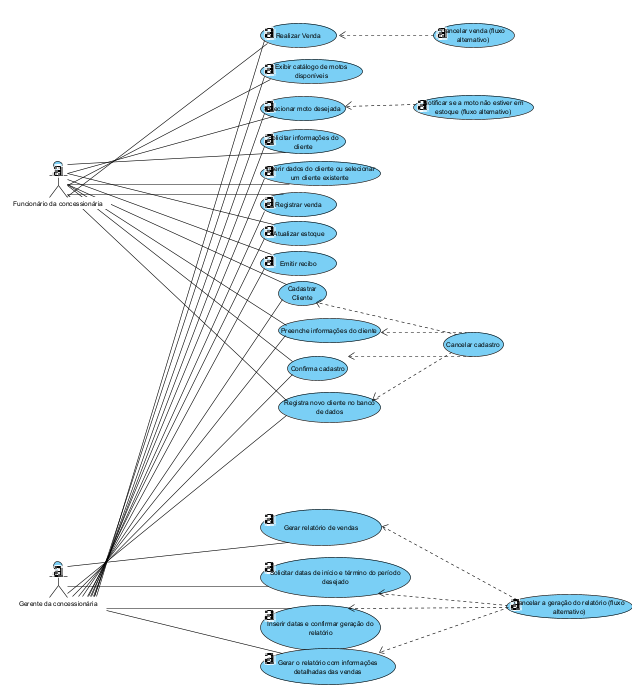
\includegraphics[width=0.7\textwidth]{diagramacaso.png}
	\caption{Diagrama de casos de uso}
	\label{fig:Diagrama de casos de uso}
\end{figure}

\subsection{Descrição dos Casos de Uso}

A seguir, são apresentados os principais casos de uso do sistema:

\subsubsection{Cadastrar Cliente}

\begin{itemize}
	\item \textbf{Ator Principal:} Funcionário da concessionária
	\item \textbf{Descrição:} Este caso de uso descreve o processo de cadastro de um novo cliente no sistema. O funcionário da concessionária insere as informações do cliente, como nome, endereço e contato.
	\item \textbf{Fluxo Básico:}
	\begin{enumerate}
		\item O funcionário seleciona a opção "Cadastrar Cliente" no sistema.
		\item O sistema exibe o formulário de cadastro de cliente.
		\item O funcionário preenche as informações do cliente.
		\item O funcionário confirma o cadastro.
		\item O sistema registra o novo cliente no banco de dados.
	\end{enumerate}
	\item \textbf{Fluxos Alternativos:}
	\begin{itemize}
		\item Em qualquer etapa do fluxo básico, o funcionário pode cancelar o cadastro.
	\end{itemize}
\end{itemize}

\subsubsection{Realizar Venda}

\begin{itemize}
	\item \textbf{Ator Principal:} Funcionário da concessionária
	\item \textbf{Descrição:} Este caso de uso descreve o processo de realização de uma venda de motos para um cliente. O funcionário da concessionária registra os itens vendidos e conclui a transação.
	\item \textbf{Fluxo Básico:}
	\begin{enumerate}
		\item O funcionário seleciona a opção "Realizar Venda" no sistema.
		\item O sistema exibe o catálogo de motos disponíveis.
		\item O funcionário seleciona a moto desejada.
		\item O sistema solicita as informações do cliente.
		\item O funcionário insere os dados do cliente ou seleciona um cliente existente.
		\item O sistema registra a venda, atualiza o estoque e emite um recibo.
	\end{enumerate}
	\item \textbf{Fluxos Alternativos:}
	\begin{itemize}
		\item Se a moto desejada não estiver em estoque, o sistema notifica o funcionário.
		\item O funcionário pode cancelar a venda em qualquer etapa.
	\end{itemize}
\end{itemize}

\subsubsection{Gerar Relatório de Vendas}

\begin{itemize}
	\item \textbf{Ator Principal:} Gerente da concessionária
	\item \textbf{Descrição:} Este caso de uso descreve como o gerente pode gerar relatórios de vendas para análise. O sistema gera um relatório que inclui informações sobre as vendas realizadas em um período específico.
	\item \textbf{Fluxo Básico:}
	\begin{enumerate}
		\item O gerente seleciona a opção "Gerar Relatório de Vendas" no sistema.
		\item O sistema solicita as datas de início e término do período desejado.
		\item O gerente insere as datas e confirma a geração do relatório.
		\item O sistema gera o relatório com informações detalhadas das vendas.
	\end{enumerate}
	\item \textbf{Fluxos Alternativos:}
	\begin{itemize}
		\item O gerente pode cancelar a geração do relatório em qualquer etapa.
	\end{itemize}
\end{itemize}

\subsection{Resumo dos Casos de Uso}

Os casos de uso apresentados nesta seção desempenham um papel fundamental no sistema de gerenciamento de concessionárias de motos. Eles representam as funcionalidades essenciais que são necessárias para o pleno funcionamento do sistema. Além disso, esses casos de uso são projetados para atender às necessidades dos diversos usuários envolvidos no processo.

Essencialmente, esses casos de uso são a espinha dorsal do sistema, abrangendo desde o processo de cadastro de clientes até a realização de vendas e a análise de desempenho. Eles desempenham um papel central na garantia de que as operações da concessionária sejam eficientes e eficazes.


\section{Modelagem do Sistema}

Nesta seção, abordaremos a modelagem do sistema de gerenciamento de concessionárias de motos. A modelagem desempenha um papel fundamental no processo de desenvolvimento de software, permitindo uma compreensão mais clara da estrutura e do funcionamento do sistema.

\subsection{Modelagem de Processos}

A modelagem de processos visa representar visualmente os fluxos de trabalho e as interações que ocorrem dentro do sistema. Isso nos ajuda a entender como as tarefas são executadas e como os diferentes elementos do sistema se relacionam. Para o sistema de gerenciamento de concessionárias de motos, realizamos a modelagem de processos que descreve as principais etapas, interações e decisões envolvidas no processo de venda, desde o atendimento ao cliente até o fechamento da venda.

\subsubsection{Diagrama de Fluxo de Trabalho da Venda}

Um dos aspectos críticos do sistema é o processo de venda de motos. O diagrama de fluxo de trabalho da venda ilustra como um cliente é atendido, como suas necessidades são identificadas, como as informações sobre motos disponíveis são apresentadas e como a venda é finalizada.

\begin{figure}[h]
	\centering
	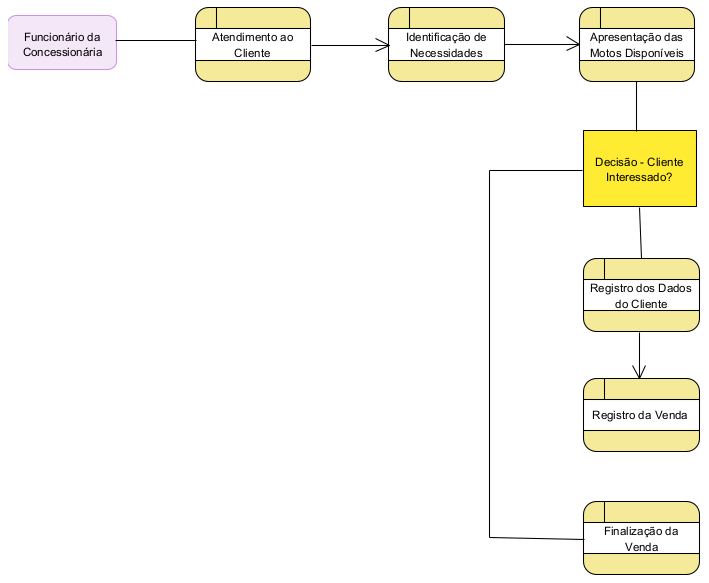
\includegraphics[width=0.7\textwidth]{diagrama-vendas.png}
	\caption{Diagrama de Fluxo de Trabalho da Venda}
	\label{fig:Diagrama de Fluxo de Trabalho da Venda}
\end{figure}

Este diagrama nos fornece uma visão geral do processo de venda e ajuda na identificação de áreas que podem ser otimizadas para melhorar a eficiência e a experiência do cliente.

Os principais componentes do diagrama são os seguintes:

\begin{itemize}
	\item \textbf{Funcionário da Concessionária (Ator Principal)}: Representa o funcionário responsável por conduzir o processo de venda.
	
	\item \textbf{Atendimento ao Cliente (Processo)}: O funcionário inicia o atendimento ao cliente quando este entra na concessionária.
	
	\item \textbf{Identificação de Necessidades (Processo)}: O funcionário identifica as necessidades e preferências do cliente em relação às motos disponíveis.
	
	\item \textbf{Apresentação das Motos Disponíveis (Processo)}: O funcionário apresenta as motos disponíveis que correspondem às necessidades do cliente.
	
	\item \textbf{Decisão - Cliente Interessado? (Decisão)}: O funcionário verifica se o cliente está interessado em fazer uma compra.
	
	\item \textbf{Registro dos Dados do Cliente (Processo)}: Se o cliente estiver interessado, o funcionário registra os dados do cliente, incluindo nome, endereço e informações de contato.
	
	\item \textbf{Registro da Venda (Processo)}: O funcionário registra a venda, incluindo as motos vendidas e o valor total.
	
	\item \textbf{Finalização da Venda (Processo)}: O funcionário conclui a venda, emite um recibo e entrega a moto ao cliente.
\end{itemize}

No fluxo básico do processo:

\begin{enumerate}
	\item O funcionário inicia o atendimento ao cliente.
	\item O funcionário identifica as necessidades do cliente.
	\item As motos disponíveis são apresentadas ao cliente.
	\item O funcionário verifica se o cliente está interessado.
	\item Se o cliente estiver interessado, o funcionário registra os dados do cliente.
	\item Em seguida, o funcionário registra a venda e a finaliza.
	\item Se o cliente não estiver interessado, o atendimento é encerrado.
\end{enumerate}


\subsection{Modelagem de Dados}

A modelagem de dados é fundamental para entender como as informações são estruturadas e armazenadas no sistema. Para o sistema de gerenciamento de concessionárias de motos, utilizamos um banco de dados relacional para armazenar dados sobre clientes, motos, vendas e outros elementos essenciais. A seguir, descrevemos as principais entidades e seus relacionamentos no modelo de dados.

\subsubsection{Entidades e Relacionamentos}

\begin{itemize}
	\item \textbf{Cliente:} Representa informações sobre os clientes da concessionária, incluindo nome, endereço e informações de contato.
	\item \textbf{Moto:} Armazena detalhes das motos disponíveis na concessionária, como marca, modelo, ano e preço.
	\item \textbf{Venda:} Registra informações sobre as vendas realizadas, incluindo data, cliente associado e itens vendidos.
\end{itemize}

O modelo de dados também inclui relacionamentos entre essas entidades, como a associação de uma venda a um cliente e a motos específicas.

\subsubsection{Diagrama de Banco de Dados}

O diagrama de banco de dados fornece uma representação visual do modelo de dados e de seus relacionamentos. Isso ajuda na implementação do banco de dados e no entendimento das consultas necessárias para acessar as informações de maneira eficaz.

\begin{figure}[h]
	\centering
	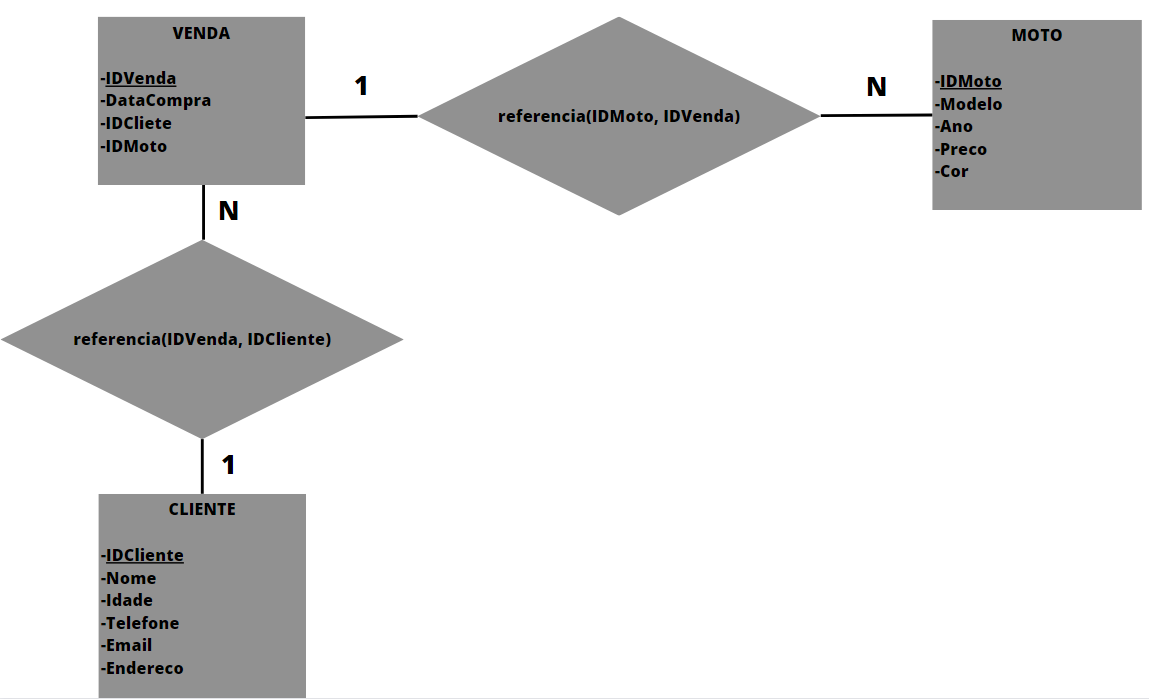
\includegraphics[width=0.7\textwidth]{banco-de-dados.png}
	\caption{Diagrama de Banco de Dados}
	\label{fig:Diagrama de Banco de Dados}
\end{figure}

O diagrama de banco de dados nos auxilia na implementação adequada do sistema de gerenciamento de concessionárias de motos e na garantia de que as informações sejam armazenadas e recuperadas de maneira eficiente.

\subsection{Resumo da Modelagem}

A modelagem do sistema é uma parte fundamental do processo de desenvolvimento do sistema de gerenciamento de concessionárias de motos. Compreende duas vertentes: a modelagem de processos e a modelagem de dados. A modelagem de processos nos permite visualizar os fluxos de trabalho, as interações e as decisões envolvidas em atividades cruciais, como vendas e relatórios. Isso ajuda a identificar áreas que podem ser otimizadas. A modelagem de dados, por outro lado, é essencial para compreender a estrutura e o armazenamento de informações, destacando entidades-chave, como clientes, motos e vendas, e seus relacionamentos. Através de um diagrama de banco de dados, conseguimos representar visualmente essas informações e suas interações. O conjunto de modelagem é valioso para a implementação adequada do sistema e garante que as informações sejam gerenciadas eficazmente. A próxima etapa envolverá testes e validação para assegurar o desempenho e a funcionalidade adequados do sistema.


